\documentclass{article}
\usepackage[margin=1.25in]{geometry}
%\usepackage[hmargin=1.25in,vmargin=1in]{geometry}

\usepackage{amsmath}
\usepackage{listings, xcolor}
\usepackage{graphicx}
\usepackage[pdfborder=000]{hyperref}
\usepackage{subfig}
\usepackage{booktabs}

\title{CLab-4 Report}
\author{Jeff Yuanbo Han\quad u6617017}
\date{May 13, 2018}

\graphicspath{{figures/task1/}{figures/task2/}}

\lstset{
	columns=fixed,
	numbers=left,
	frame=none,
	keywordstyle=\color[RGB]{40,40,255},
	numberstyle=\footnotesize\color{darkgray},
	commentstyle=\it\color[RGB]{0,96,96},
	stringstyle=\rmfamily\slshape\color[RGB]{128,0,0},
	showstringspaces=false,
	language=Python,
}

\begin{document}
\maketitle

In computer lab 4, I experiment both tasks. And My major task is CNN (deep learning) for MNIST handwritten digit recognition; Task 2---Camera calibration will serve as a bonus.

\tableofcontents


\section{CNN Based Vision Recognition}
\subsection{My CNN Model}
To achieve the goal of recognizing MNIST handwritten digits, I have tried tens of neural networks, ranging from the basic single-layer net to the classic LeNet-5. However, the most effective architectures usually involves more than 3 hidden layers, and therefore is quite time-consuming. The guideline of CLab-4 requires our model to limit training procedure to 3 minutes. So I have to prune those subtle but complex structures. After myriads of experiments, I finally choose my deep neural network as the one contain a convolutional layer and a full-connected layer:

\begin{center}
	\begin{tabular}{lcr}
		\toprule
		Layer & Window Size & Features/Units \\
		\midrule
		Input & $28\times28$ & 1 \\
		Convolution & $5\times5$ & 6 \\
		Max-pool & $2\times2$ & 6 \\
		Full-connected & 1 & 300 \\
		Output & 1 & 10 \\
		\bottomrule
	\end{tabular}
\end{center}

All the activation functions are using ReLU, i.e. Rectified Linear Unit, mathematically, $\max(0, input)$. As a result of experiments, ReLU is the most efficient among functions that are commonly used for activation (Softmax, Tanh, etc.). This means performing, say Softmax, in a 2-hidden-layer network can hardly complete training under 3 minutes.

My Settings are
\begin{equation}
\begin{aligned}
	& \text{Initializer} = \text{Trimmed Normal Distribution ($\mu=0, \sigma=0.3$)}; \\
	& \text{Batch size} = 50; \\
	& \text{Iteration} = 5000; \\
	& \text{Learning rate} = 0.001; \\
	& \text{Optimizer} = \text{Adam}; \label{base}
\end{aligned}
\end{equation}

The training time is on average 175s. And the test accuracy is usually above 90\%. With several attempts, the best run arrives at 95.33\%. This result can still be better with larger batch-size, but it will violate the rule of time. The training error descent procedure is shown below in \hyperref[fig-1]{Figure~1}. In following sections, you will see each hyper-parameter of my settings is at least a local optima to some extent, and they overall account for my choice of model.

\begin{figure}
	\centering
	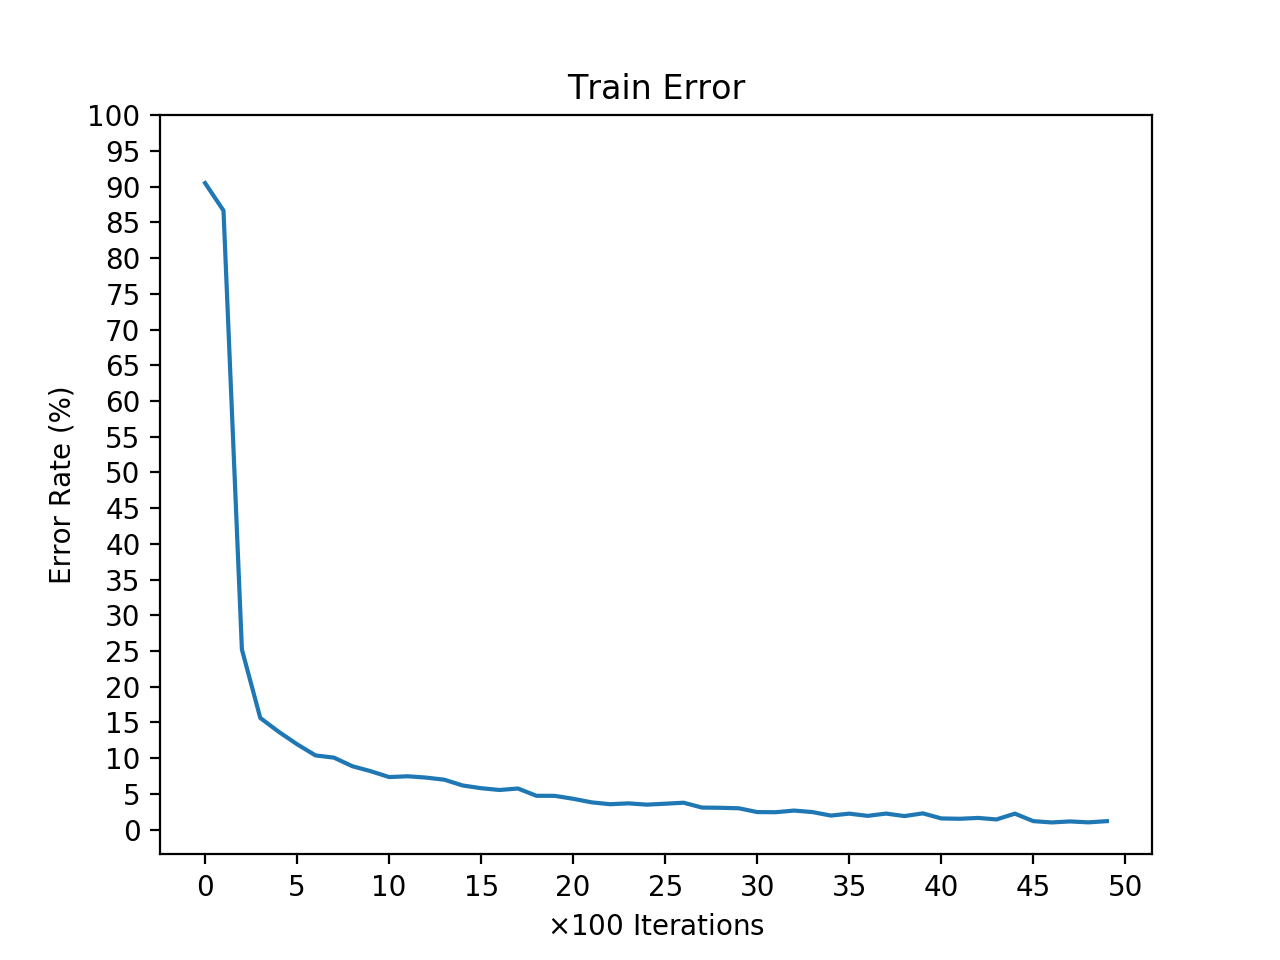
\includegraphics[scale=0.5]{my.png}
	\caption{Benchmark: my final model}
	\label{fig-1}
\end{figure}


\subsection{Batch Size}
In this section, I experiment with the batch-size. Maintaining my model architecture and all the other hyper-parameters except batch-size and iteration. When batch-size gets bigger, the epochs, which reflects the real amount of computation, will increase meanwhile. So we may have to reduce the number of iterations in order to satisfy the 3-min requirement, and vice versa (can train more steps with small batch-size). The \hyperref[tab-2]{Batch Size Table} and \hyperref[fig-2]{Figure-2} show an approximate comparison of different batch-sizes.

\begin{center}
	\label{tab-2}
	\begin{tabular}{ccc}
		\toprule
		Batch size & Iteration & Test accuracy \\
		\midrule
		10 & 6500 & 52\% \\
		50 & 5000 & 95\% \\
		100 & 3500 & 88\% \\
		200 & 2000 & 79\% \\
		\bottomrule
	\end{tabular}
\end{center}

\begin{figure}
	\centering
	\subfloat{
		\centering
		\fbox{
			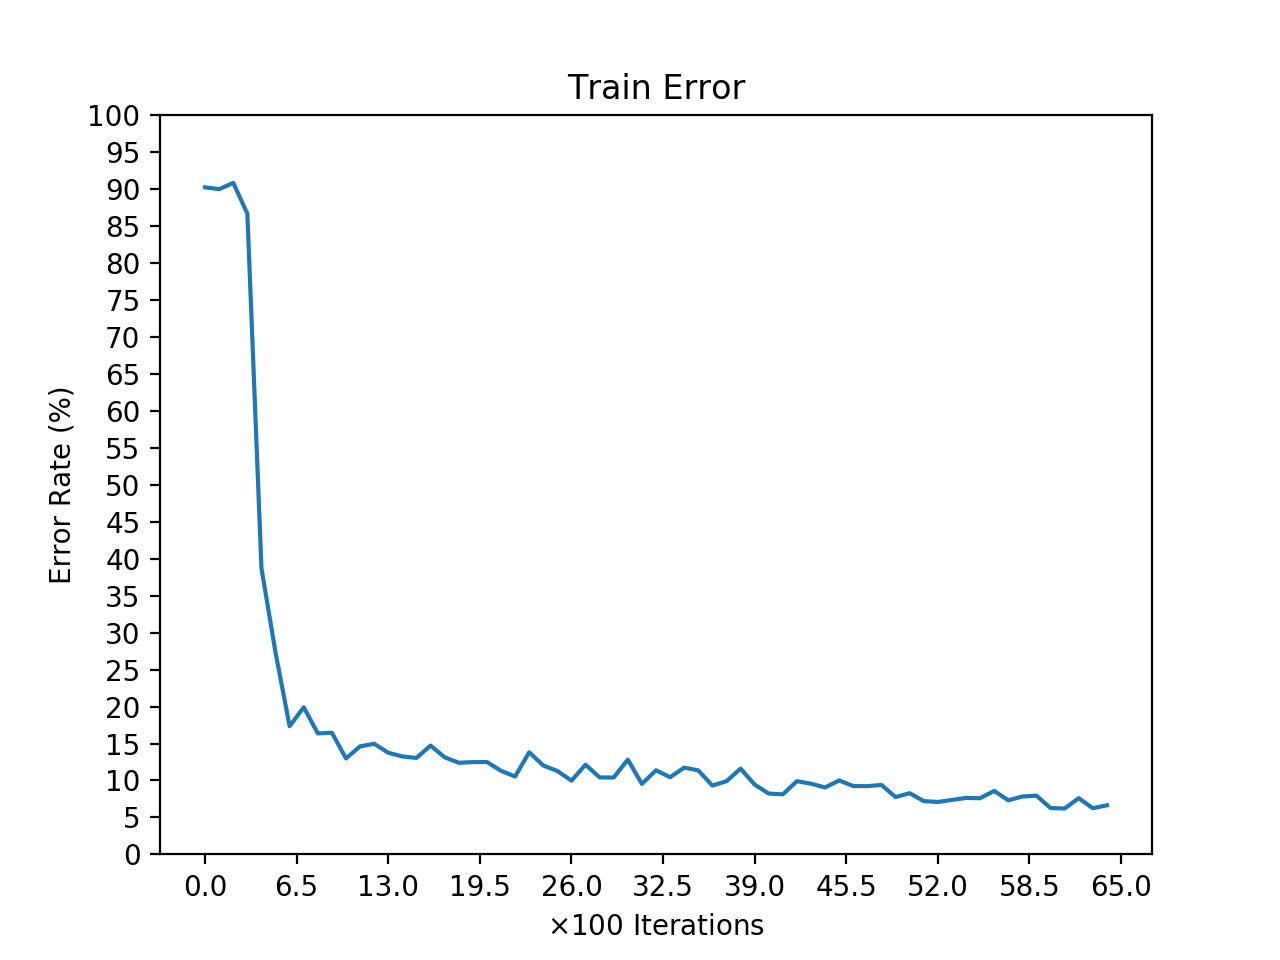
\includegraphics[scale=0.3]{batch_10.png}}
	}
	\subfloat{
		\centering
		\fbox{
			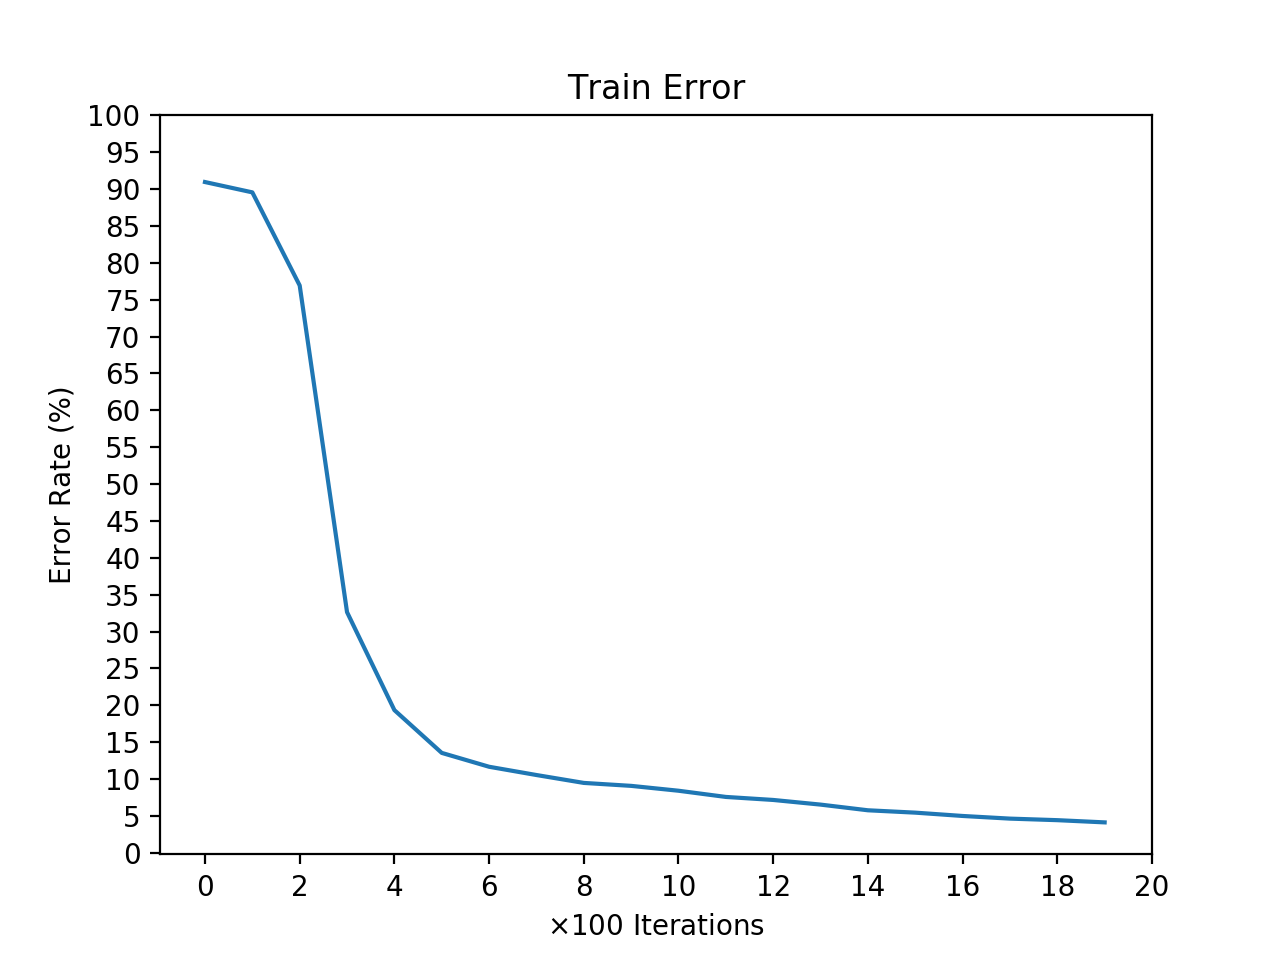
\includegraphics[scale=0.3]{batch_200.png}}
	}
	\caption{Batch size = 10 \& 200}
	\label{fig-2}
\end{figure}


\subsection{Learning Rate}
Experimenting with learning rate is much easier. Just keep the \hyperref[base]{Baseline} settings and change learning rate only. Results are displayed in the \hyperref[tab-3]{Learning Rate Table} and \hyperref[fig-3]{Figure~}. As a consequence, we could infer that learning rate $\ge 0.01$ is too big for parameters to converge, and $\le 0.001$ is so small that the model has not been trained adequately.
\begin{center}
	\label{tab-3}
	\begin{tabular}{cc}
		\toprule
		Learning rate & Test accuracy \\
		\midrule
		0.1 & 15\% \\
		0.01 & 47\% \\
		0.001 & 95\% \\
		0.0001 & 41\% \\
		\bottomrule
	\end{tabular}
\end{center}

\begin{figure}
	\centering
	\subfloat{
		\centering
		\fbox{
			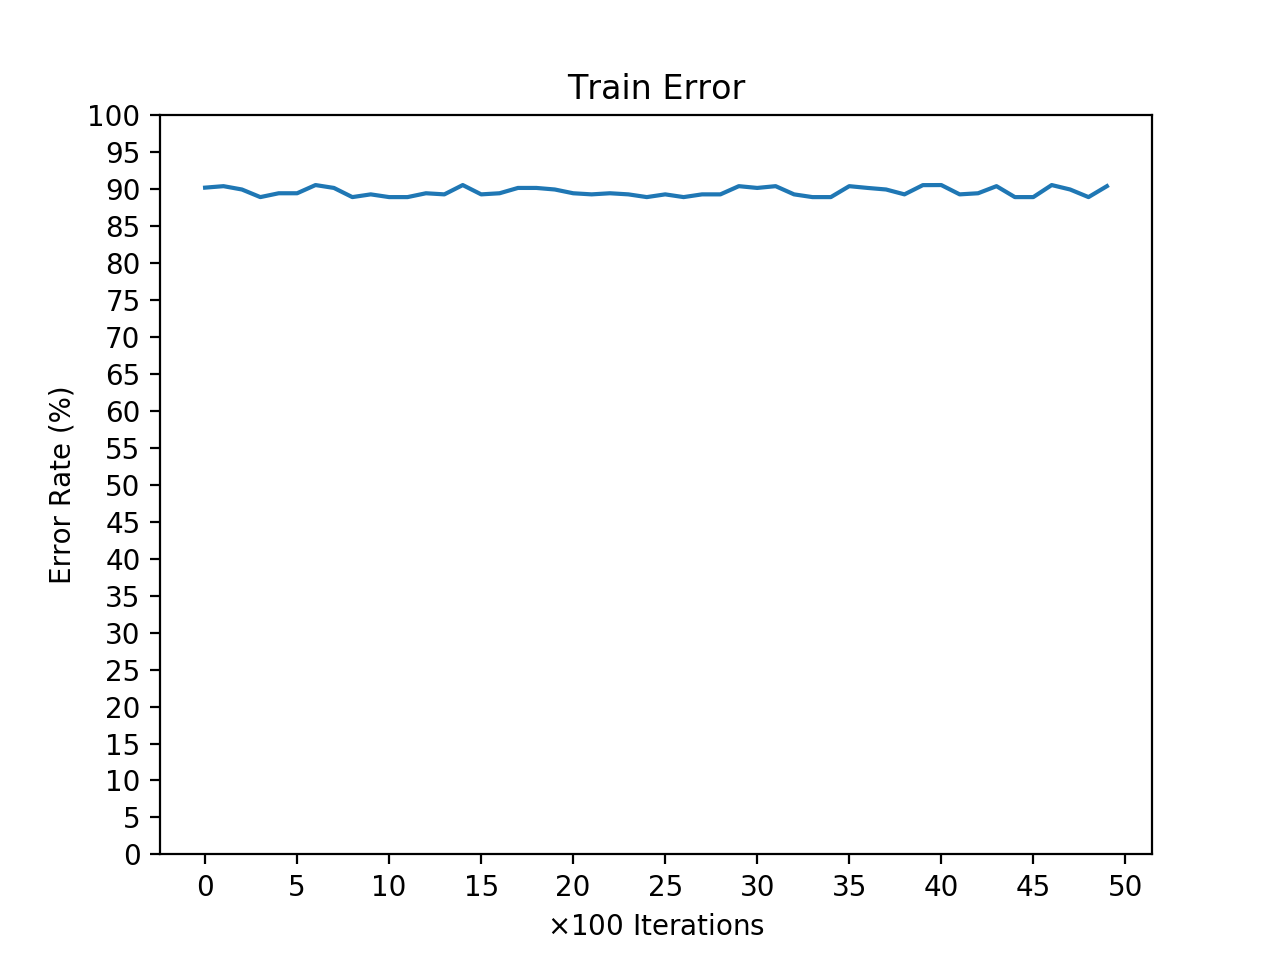
\includegraphics[scale=0.3]{lr_0.1.png}}
	}
	\subfloat{
		\centering
		\fbox{
			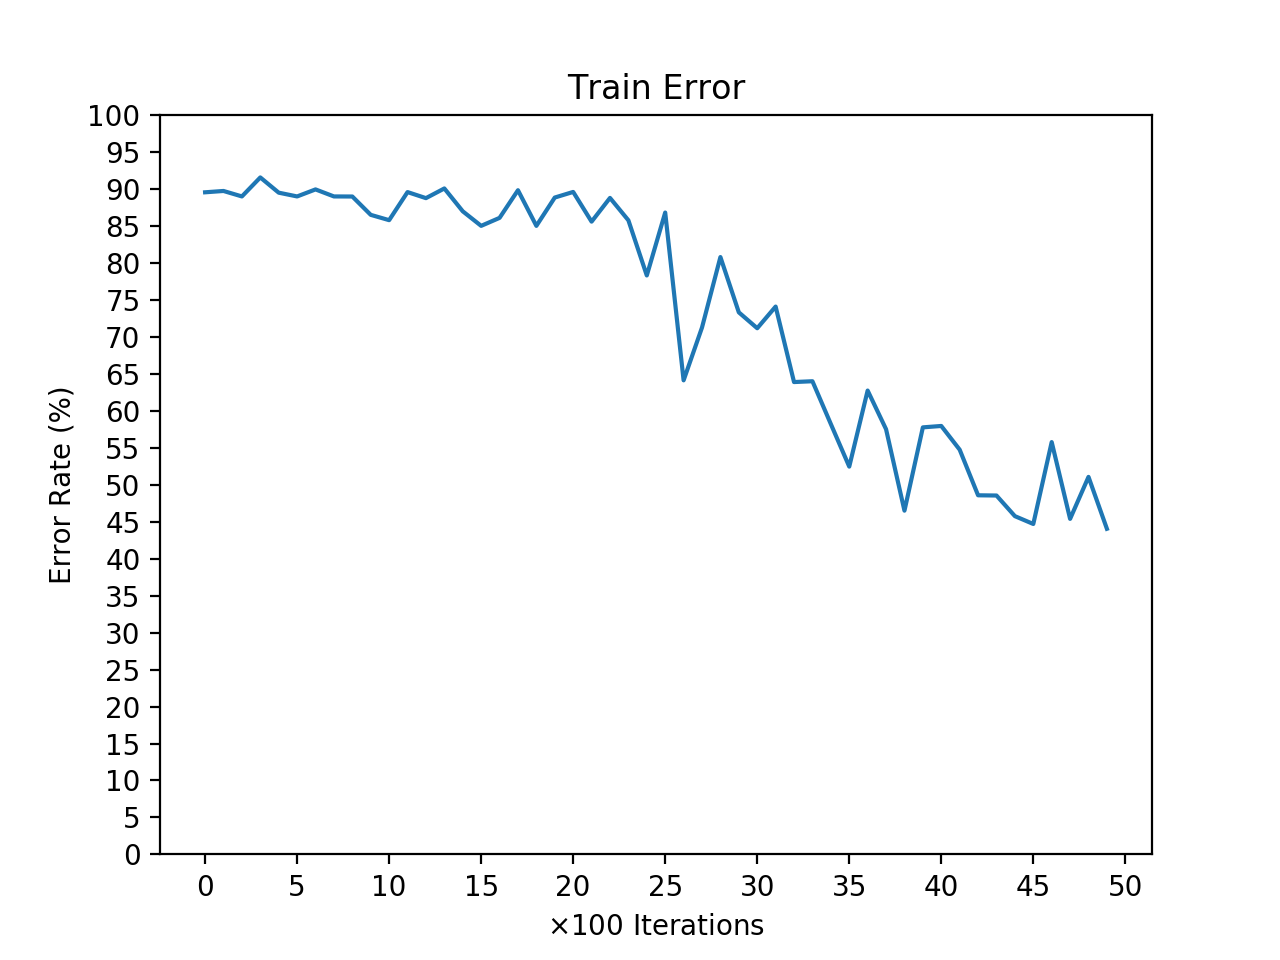
\includegraphics[scale=0.3]{lr_0.0001.png}}
	}
	\caption{Learning rate = 0.1 \& 0.0001}
	\label{fig-3}
\end{figure}


\subsection{Initializer}
Trying to change other initializers also get different outputs. Please look at the \hyperref[tab-7]{Initializer Table} and \hyperref[fig-4]{Figure~4}.
\begin{center}
	\label{tab-7}
	\begin{tabular}{ccc}
		\toprule
		Distribution & Parameter & Test accuracy \\
		\midrule
		Trimmed Normal & $\mu=0,\sigma=0.1$ & 82\% \\
		Trimmed Normal & $\mu=0,\sigma=0.3$ & 95\% \\
		Trimmed Normal & $\mu=0,\sigma=0.5$ & 84\% \\
		Uniform & [-1, 1] & 18\% \\
		Point (Constant) & 0 & 88\% \\
		\bottomrule
	\end{tabular}
\end{center}

\begin{figure}
	\centering
	\subfloat{
		\centering
		\fbox{
			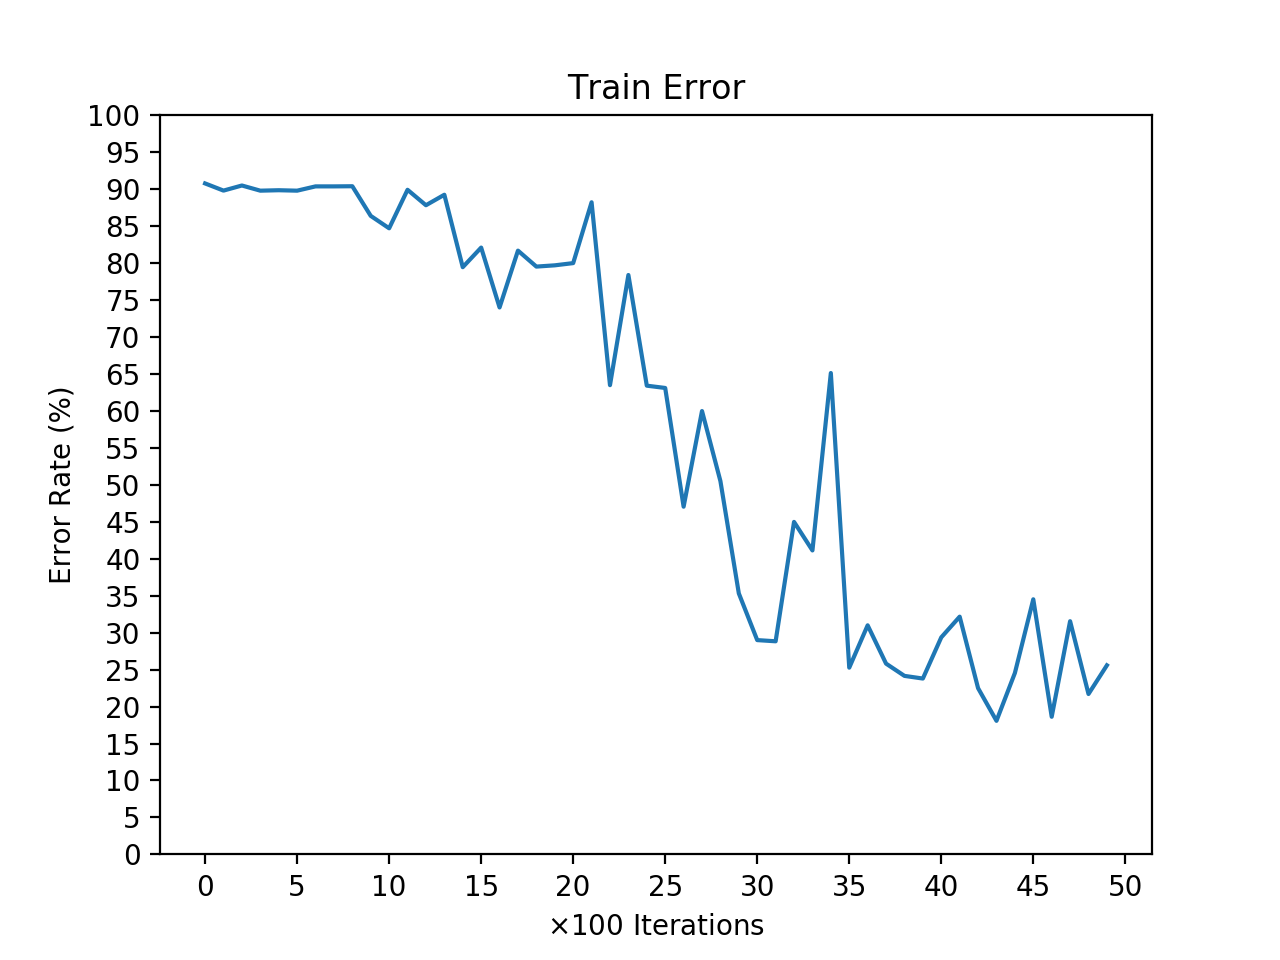
\includegraphics[scale=0.3]{uniform.png}}
	}
	\subfloat{
		\centering
		\fbox{
			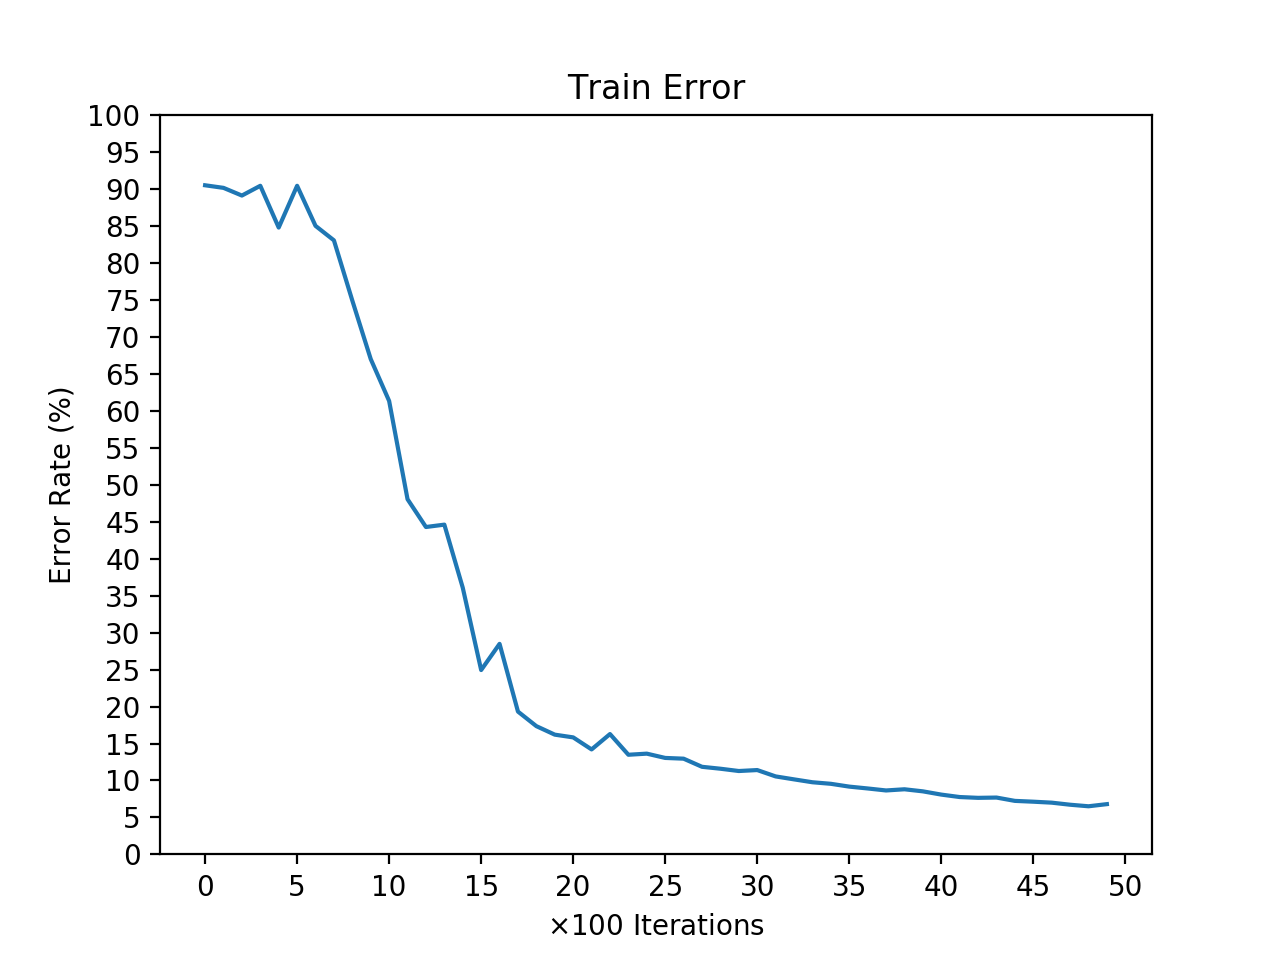
\includegraphics[scale=0.3]{const.png}}
	}
	\caption{Initializer = Uniform(-1, 1) \& Constant 0}
	\label{fig-4}
\end{figure}


\subsection{Optimizer}
Similiarly as before, remain all the other setting as \hyperref[base]{Baseline}, and then try different optimizers (see the \hyperref[tab-4]{Optimizer Table} and \hyperref[fig-5]{Figure~5}). We find that other optimizers do not agree with this specific model, possibly in that all the hyper-parameters are set and fixed under Adam optimizer.

\begin{center}
	\label{tab-4}
	\begin{tabular}{cc}
		\toprule
		Optimizer & Test accuracy \\
		\midrule
		Adam & 95\% \\
		Adagrad & 24\% \\
		SGD & 17\% \\
		\bottomrule
	\end{tabular}
\end{center}

\begin{figure}
	\centering
	\subfloat{
		\centering
		\fbox{
			\includegraphics[scale=0.3]{Adagrad.png}}
	}
	\subfloat{
		\centering
		\fbox{
			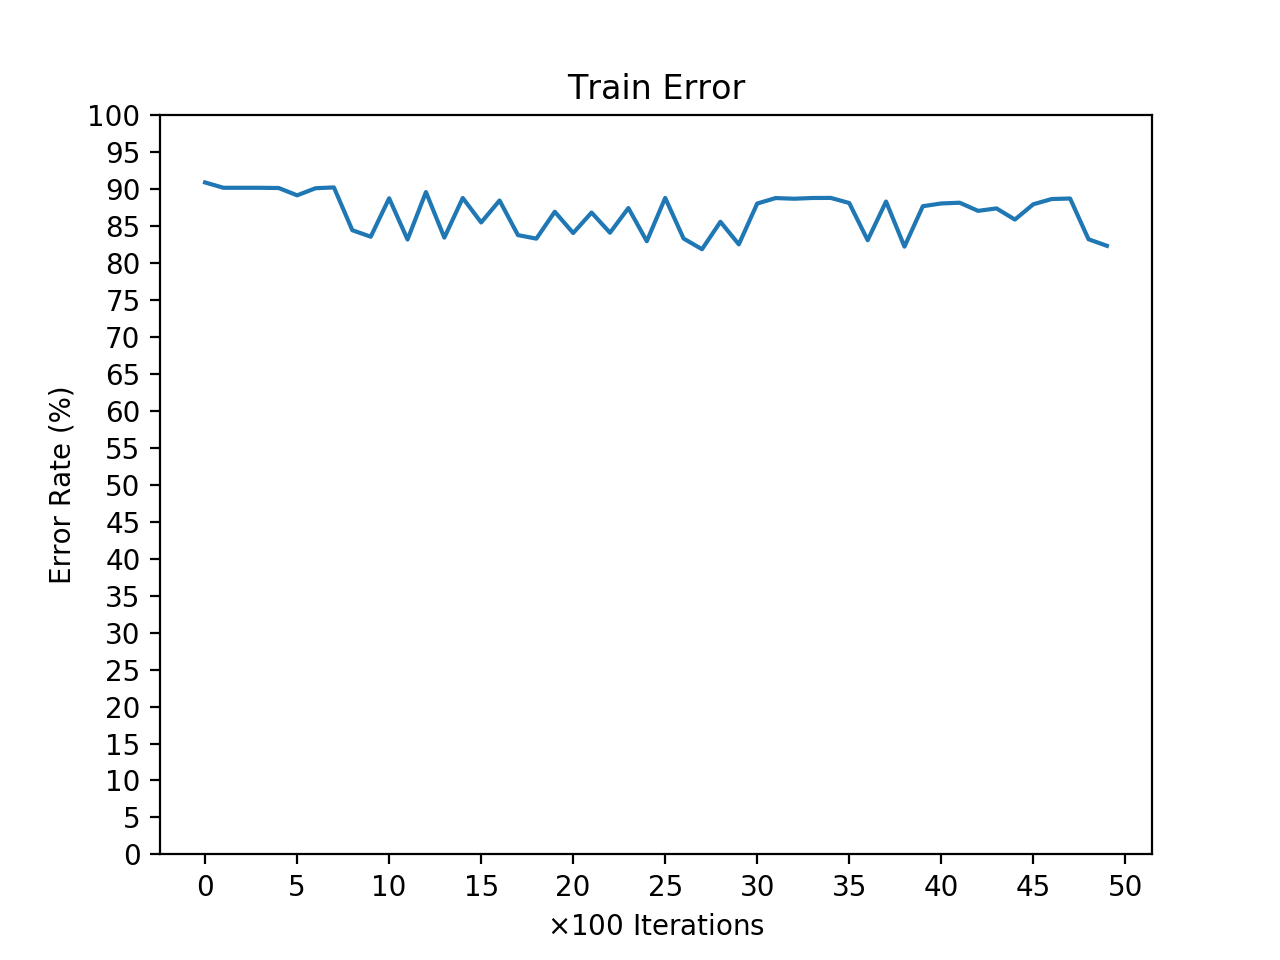
\includegraphics[scale=0.3]{SGD.png}}
	}
	\caption{Optimizer = Adagrad \& SGD}
	\label{fig-5}
\end{figure}


\subsection{Drop Out}
I am not using drop-out technique in my final model, but I do have studied on it. With drop-out rate = 0.5, the model can achieve 76\% or so test accuracy (see the \hyperref[tab-5]{Optimizer Table} and \hyperref[fig-6]{Figure~6}). In other words, the result has not been improved at least within 3 minutes; instead, it still needs a number of training processes. This is probably because our network has such an elementary topology that adopting dropout is needless.

\begin{center}
	\label{tab-5}
	\begin{tabular}{cc}
		\toprule
		Drop-out rate & Test accuracy \\
		\midrule
		0 & 95\% \\
		0.5 & 76\% \\
		\bottomrule
	\end{tabular}
\end{center}

\begin{figure}
	\centering
	\subfloat{
		\centering
		\fbox{
			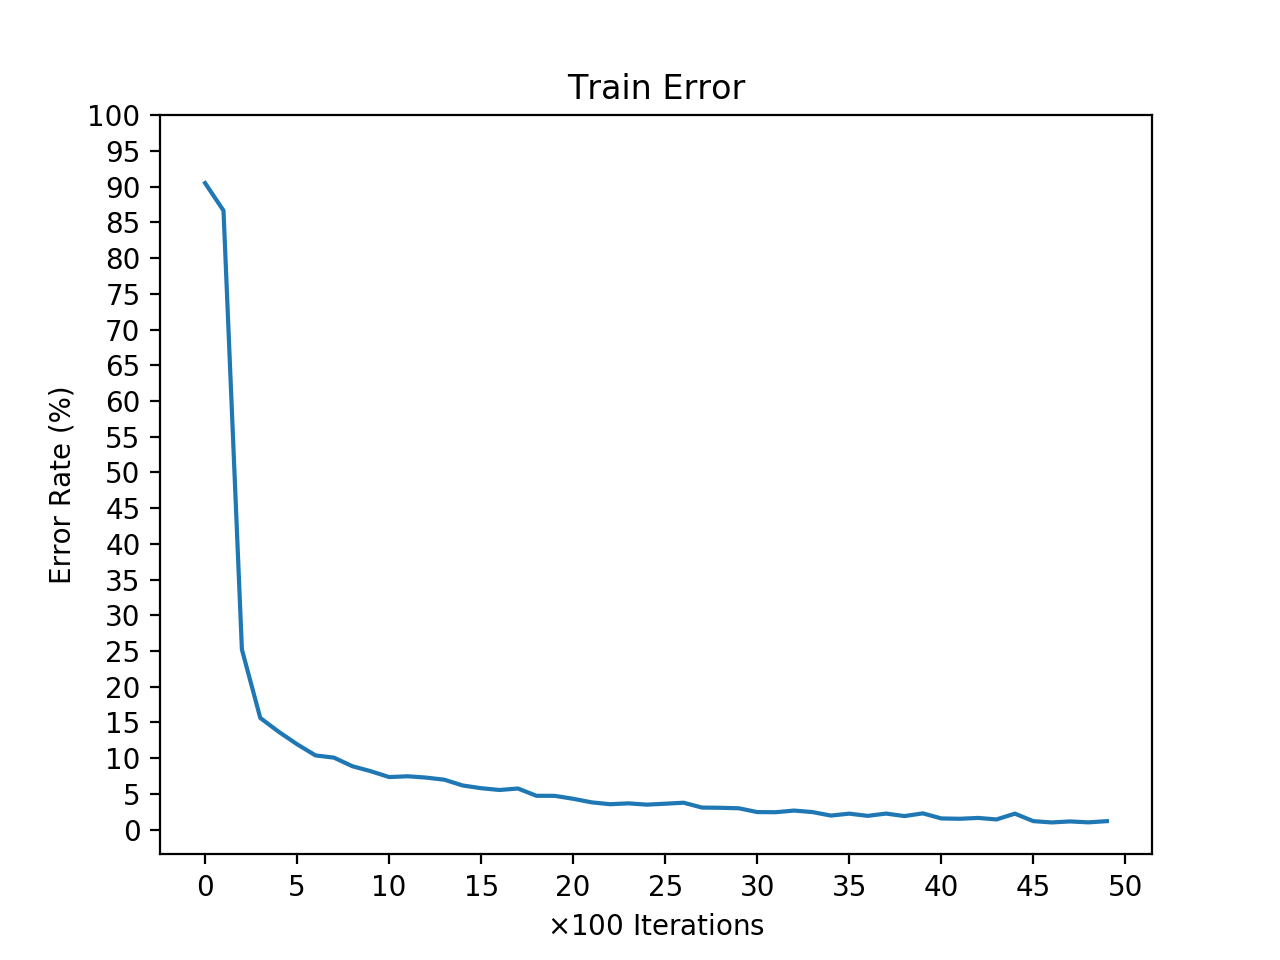
\includegraphics[scale=0.3]{my.png}}
	}
	\subfloat{
		\centering
		\fbox{
			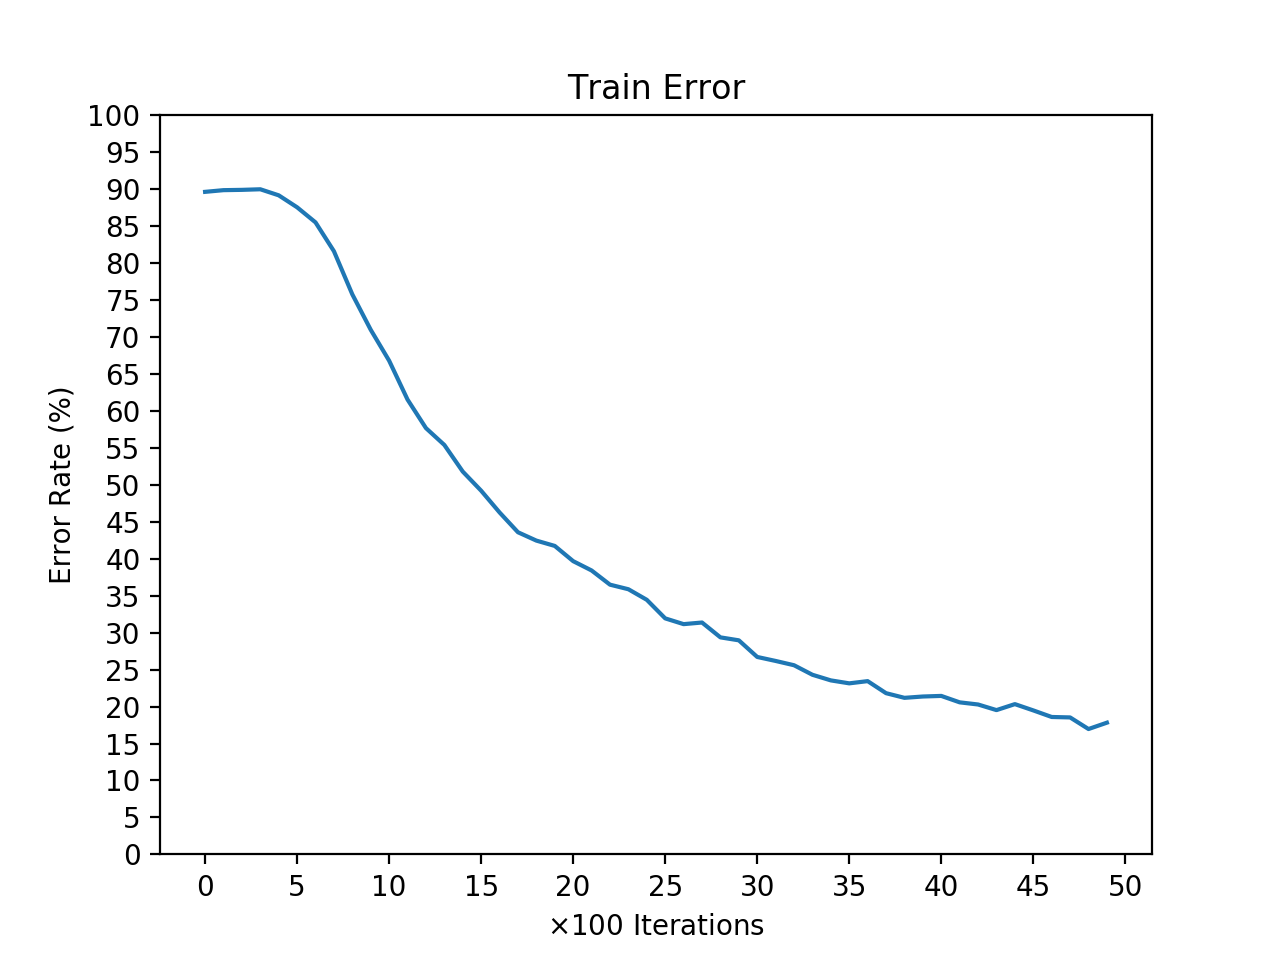
\includegraphics[scale=0.3]{drop_0.5.png}}
	}
	\caption{Drop-out rate = 0 \& 0.5}
	\label{fig-6}
\end{figure}


\subsection{Hidden Layer}
As described in Section~1.1, my final model is $cnn\_1\_1$, i.e. 1 convolutional layer (and max-pooling) + 1 full-connected layer. I have also tried 2 convolutional layers ($cnn\_2\_1$) or 2 full-connected layers ($cnn\_1\_2$). They of course have the potential to exceed $cnn\_1\_1$ theoretically. However, this is a time-limited task, so we have to cut the training iterations to accord with 3-min requirement. Under this circumstance, results are show below in the \hyperref[tab-6]{Model Table} and \hyperref[fig-7]{Figure~7}.

\begin{center}
	\label{tab-6}
	\begin{tabular}{ccccc}
		\toprule
		Model & Convolution + Max-pool & Full-connected & Iteration & Test accuracy \\
		\midrule
		$cnn\_1\_1$ & 6 features & 300 & 5000 & 95\% \\
		$cnn\_1\_2$ & 6 features & 300 + 180 &3500 & 80\% \\
		$cnn\_2\_1$ & 6 + 16 features & 180 & 3000 & 35\% \\
		\bottomrule
	\end{tabular}
\end{center}

\begin{figure}
	\centering
	\subfloat{
		\centering
		\fbox{
			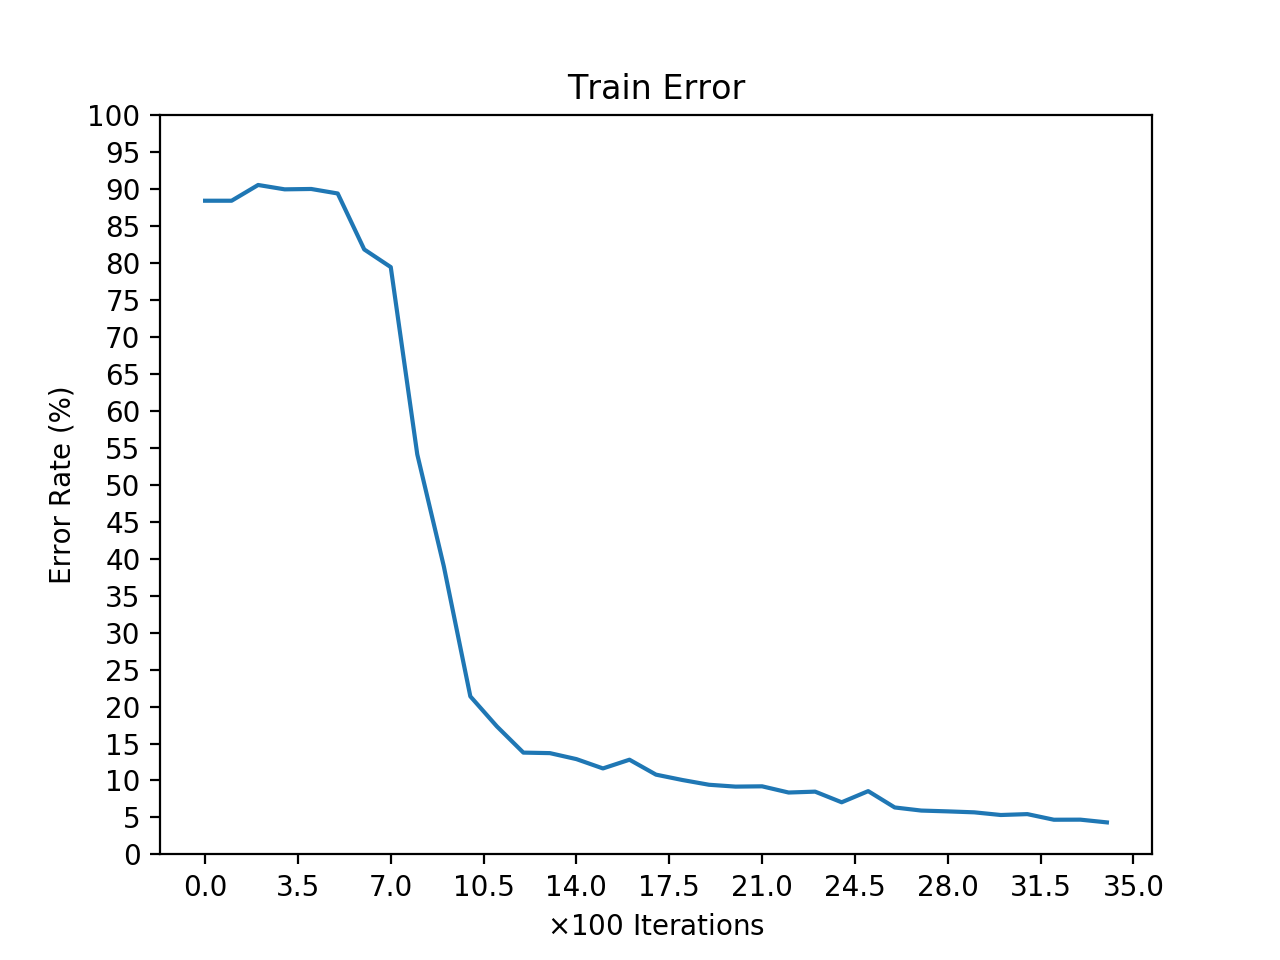
\includegraphics[scale=0.3]{cnn_1_2.png}}
	}
	\subfloat{
		\centering
		\fbox{
			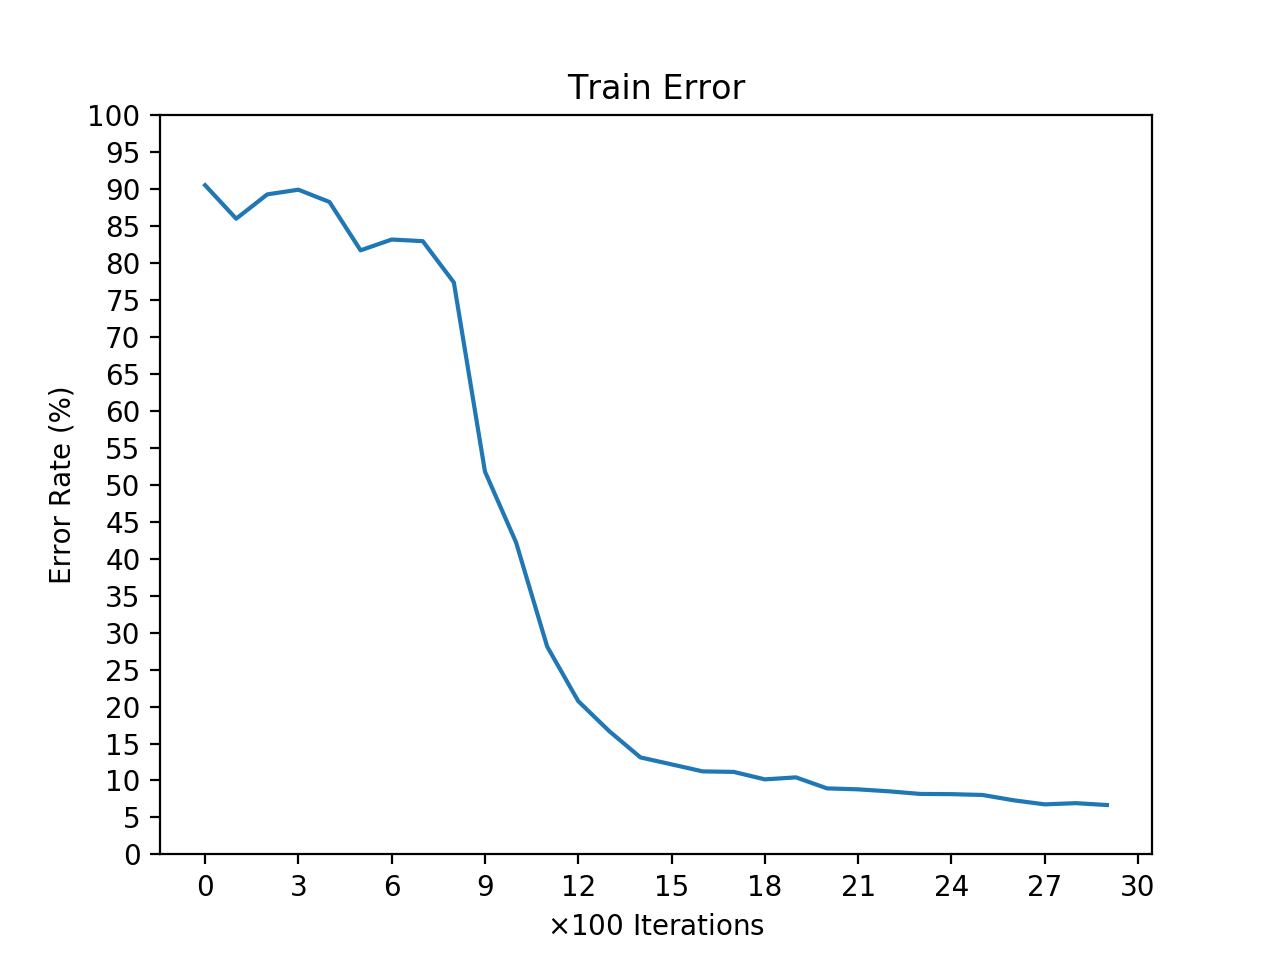
\includegraphics[scale=0.3]{cnn_2_1.png}}
	}
	\caption{$cnn\_1\_2$ \& $cnn\_2\_1$}
	\label{fig-7}
\end{figure}

In addition, $cnn\_2\_2$ becomes the classic LeNet-5\cite{LeNet}, which has obtained $99.05\%$ test accuracy, and can be better with appropriate distorted training images. However, such complicated networks are impossible to run out within 3 minutes.


\section{Camera Calibration}
\subsection{Illustration by Pictures}
My implement of estimating Calibration matrix is listed at \hyperref[code-2.1]{$calibrate.m$}. I have selected two images to check the Calibration, namely: stereo2012a.jpg and stereo2012d.jpg (\hyperref[fig-2.1]{Figure~8}). In these 2 pictures, red crosses are the points I choose originally, whereas blue circles are the estimated locations of the chosen points projected by Calibration. The green lines show the projected X, Y, Z axises.

\begin{figure}
	\centering
	\centering
	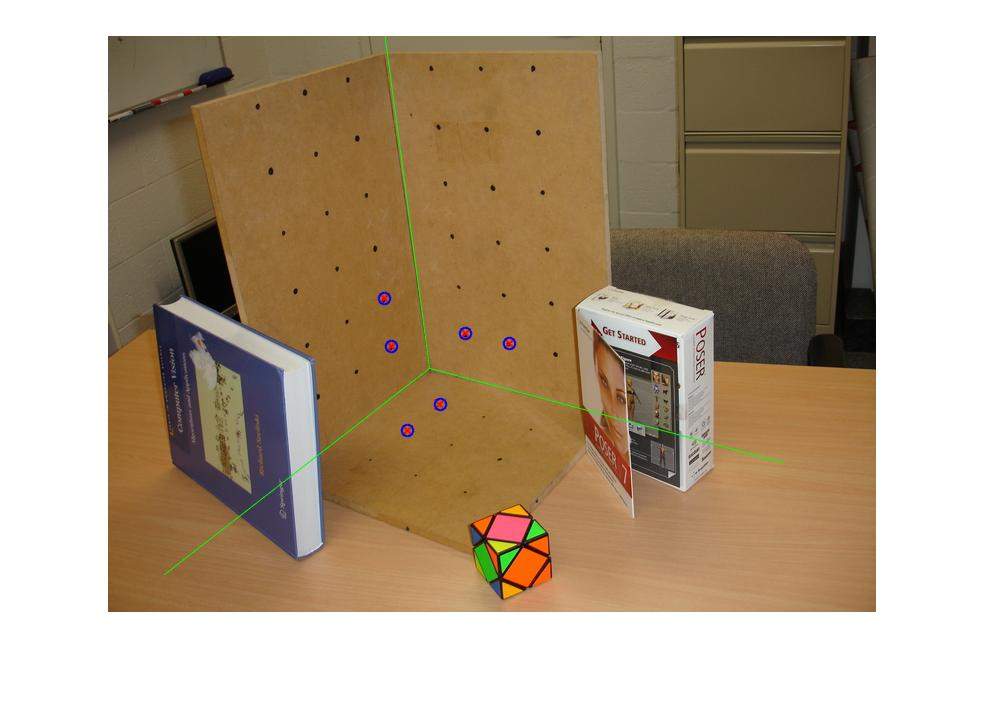
\includegraphics[scale=0.4]{a_cali.jpg}
	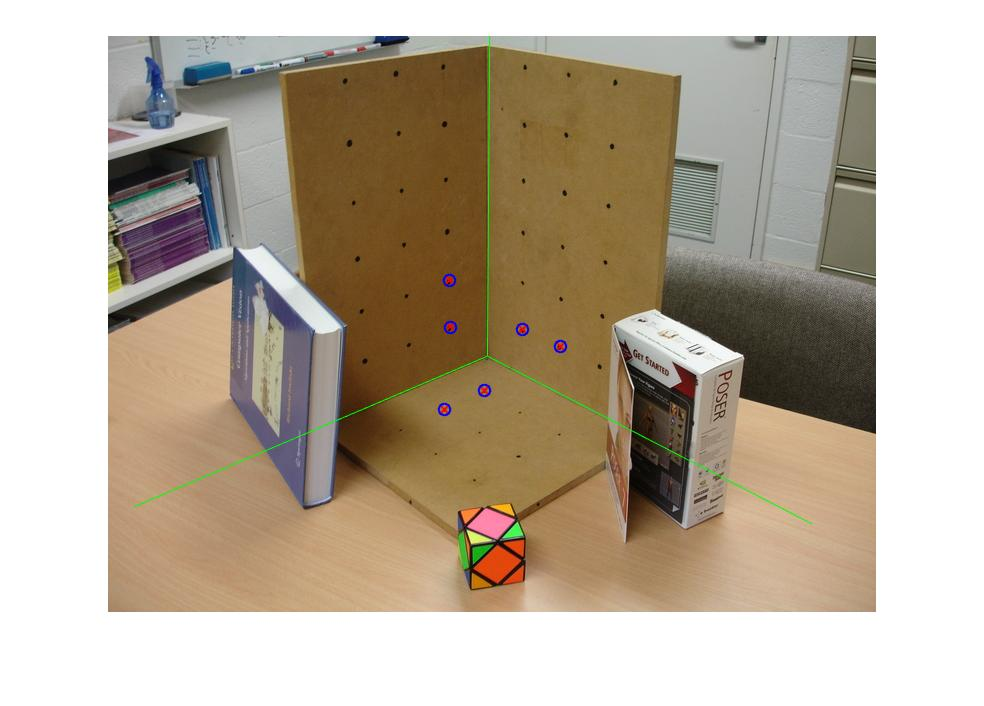
\includegraphics[scale=0.4]{d_cali.jpg}
	\caption{stereo2012a.jpg \& stereo2012d.jpg}
	\label{fig-2.1}
\end{figure}

\subsection{Calibration Data}
Take stereo2012d.jpg as an example. The outputs after running \hyperref[code-2.2]{$selectPoints.m$} and \hyperref[code-2.3]{$estimateC.m$} are:
\begin{verbatim}
MSE = 0.134857

C =

-0.0052    0.0022    0.0145   -0.7640
-0.0013    0.0141   -0.0006   -0.6448
0.0000    0.0000    0.0000   -0.0020


K =

805.6066    8.3036  414.9998
0  795.2093  216.8355
0         0    1.0000


R =

0.7064    0.0312   -0.7071
0.2711   -0.9348    0.2296
-0.6538   -0.3539   -0.6688


t =

76.1529
55.9128
71.1172
\end{verbatim}
Let $f_x$ = horizontal focal length, $f_y$ = vertical focal length, then
\begin{align*}
	f_x &= K[1,1] = 805.6066 \\
	f_y/\sin\theta &= K[2,2] = 795.2093 \\
	-f_x\cot\theta &= K[1,2] = 8.3036
\end{align*}
Solving them, we derive
\begin{align*}
	f_x &= 805.6066 \\
	f_y &= 795.1671
\end{align*}
Besides, it is not hard to know
\[
\sin \alpha_y = R[1,3] = -0.7071
\]
Thus we obtain
\[
\alpha_y = -0.7854 \text{ rad} \approx -45^\circ \text{ degree}
\]
which is the pitch angle of camera with respect to X-Z plane in the world coordinate system.


\begin{thebibliography}{1}
	\bibitem{LeNet} Lecun, Y., Bottou, L., Bengio, Y., \& Haffner, P. (1998). Gradient-based learning applied to document recognition. Proceedings of the IEEE, 86(11), 2278-2324.
\end{thebibliography}


\appendix
\section{Python \& MATLAB Codes}

\subsection{CNN Based Vision Recognition}
\subsubsection{$cnn\_1\_1.py$}
\label{code-1}
\begin{lstlisting}
# -*- coding: utf-8 -*-
"""
1 * (Convolution + Max_pool) + 1 * Full-connected
"""
import tensorflow as tf
from tensorflow.examples.tutorials.mnist import input_data
from random import sample
import matplotlib.pyplot as plt
from time import time


def weight_variable(shape):
initial = tf.truncated_normal(shape, stddev=0.3)
#initial = tf.random_uniform(shape=shape, minval=-1, maxval=1)
return tf.Variable(initial)


def bias_variable(shape):
#initial = tf.constant(0.1, shape=shape)
#initial = tf.random_uniform(shape=shape, minval=-1, maxval=1)
initial = tf.truncated_normal(shape, stddev=0.3)
return tf.Variable(initial)


def conv2d(x, W):
return tf.nn.conv2d(x, W, strides=[1, 1, 1, 1], padding='VALID')


def max_pool_2x2(x):
return tf.nn.max_pool(x, ksize=[1, 2, 2, 1],
strides=[1, 2, 2, 1], padding='VALID')


if __name__ == '__main__':
# Read in MNIST data
mnist = input_data.read_data_sets("MNIST_data/", one_hot=True)
ind = sample(range(mnist.train.images.shape[0]), 10000)
train = tf.contrib.learn.datasets.mnist.DataSet(
mnist.train.images[ind,:], mnist.train.labels[ind,:], one_hot=True, reshape=False)

# Placeholders of training attributes and labels
x = tf.placeholder(tf.float32, [None, 784])
y_ = tf.placeholder(tf.float32, [None, 10])

# Reshape images from 728*1 to 28*28
x_image = tf.reshape(x, [-1, 28, 28, 1])

# Convolutional layer
W_conv1 = weight_variable([5, 5, 1, 6])
b_conv1 = bias_variable([6])
h_conv1 = tf.nn.relu(conv2d(x_image, W_conv1) + b_conv1)
h_pool1 = max_pool_2x2(h_conv1)

# Full-connected layer, ReLU
W_fc1 = weight_variable([12 * 12 * 6, 300])
b_fc1 = bias_variable([300])
h_pool1_flat = tf.reshape(h_pool1, [-1, 12 * 12 * 6])
h_fc1 = tf.nn.relu(tf.matmul(h_pool1_flat, W_fc1) + b_fc1)

# Placeholder of keep_prob for dropout
keep_prob = tf.placeholder(tf.float32)

# Output layer with 10 classes
W_fc2 = weight_variable([300, 10])
b_fc2 = bias_variable([10])
h_fc1_drop = tf.nn.dropout(h_fc1, keep_prob)
y_conv = tf.matmul(h_fc1_drop, W_fc2) + b_fc2

# Compute cost: Cross entropy after softmax
cross_entropy = tf.reduce_mean(
tf.nn.softmax_cross_entropy_with_logits(labels=y_, logits=y_conv))

# Learning step, optimized by Adam
train_step = tf.train.AdamOptimizer(1e-3, 0).minimize(cross_entropy)

# Define accuracy
correct_prediction = tf.equal(tf.argmax(y_conv, 1), tf.argmax(y_, 1))
accuracy = tf.reduce_mean(tf.cast(correct_prediction, tf.float32))

# Create Session and initialize variables
sess = tf.InteractiveSession()
sess.run(tf.global_variables_initializer())

# Training process
iteration = 5000
err = []
start_time = time()
for i in range(iteration):
batch = train.next_batch(50)
# Report the accuracy on training set every 100 steps
if i % 100 == 0:
train_accuracy = accuracy.eval(feed_dict={
x: train.images, y_: train.labels, keep_prob: 1.0})
print("step %d, train accuracy %g" % (i, train_accuracy))
err.append(1-train_accuracy)
train_step.run(feed_dict={x: batch[0], y_: batch[1], keep_prob: 1.0})

end_time = time()
print('Training time: {}s'.format(end_time-start_time))

# Accuracy on test set
print("test accuracy %g" % accuracy.eval(feed_dict={
x: mnist.test.images, y_: mnist.test.labels, keep_prob: 1.0}))

# Plot training error
plt.plot(range(len(err)), err)
plt.title('Train Error')
plt.xlabel(r'$\times100$ Iterations')
plt.ylabel('Error Rate (%)')
plt.xticks([i*iteration/1000 for i in range(11)])
plt.yticks([e*0.05 for e in range(21)], [e*5 for e in range(21)])
plt.show()

\end{lstlisting}


\subsubsection{$cnn\_1\_2.py$}
\label{code-2}
\begin{lstlisting}
# -*- coding: utf-8 -*-
"""
1 * (Convolution + Max_pool) + 2 * Full-connected
"""
import tensorflow as tf
from tensorflow.examples.tutorials.mnist import input_data
from random import sample
import matplotlib.pyplot as plt
from time import time


def weight_variable(shape):
initial = tf.truncated_normal(shape, stddev=0.3)
#initial = tf.random_uniform(shape=shape, minval=-1, maxval=1)
return tf.Variable(initial)


def bias_variable(shape):
#initial = tf.constant(0.1, shape=shape)
#initial = tf.random_uniform(shape=shape, minval=-1, maxval=1)
initial = tf.truncated_normal(shape, stddev=0.3)
return tf.Variable(initial)


def conv2d(x, W):
return tf.nn.conv2d(x, W, strides=[1, 1, 1, 1], padding='VALID')


def max_pool_2x2(x):
return tf.nn.max_pool(x, ksize=[1, 2, 2, 1],
strides=[1, 2, 2, 1], padding='VALID')


if __name__ == '__main__':
# Read in MNIST data
mnist = input_data.read_data_sets("MNIST_data/", one_hot=True)
ind = sample(range(mnist.train.images.shape[0]), 10000)
train = tf.contrib.learn.datasets.mnist.DataSet(
mnist.train.images[ind,:], mnist.train.labels[ind,:], one_hot=True, reshape=False)

# Placeholders of training attributes and labels
x = tf.placeholder(tf.float32, [None, 784])
y_ = tf.placeholder(tf.float32, [None, 10])

# Reshape images from 728*1 to 28*28
x_image = tf.reshape(x, [-1, 28, 28, 1])

# Convolutional layer
W_conv1 = weight_variable([5, 5, 1, 6])
b_conv1 = bias_variable([6])
h_conv1 = tf.nn.relu(conv2d(x_image, W_conv1) + b_conv1)
h_pool1 = max_pool_2x2(h_conv1)

# Full-connected layer 1, ReLU
W_fc1 = weight_variable([12 * 12 * 6, 300])
b_fc1 = bias_variable([300])
h_pool1_flat = tf.reshape(h_pool1, [-1, 12 * 12 * 6])
h_fc1 = tf.nn.relu(tf.matmul(h_pool1_flat, W_fc1) + b_fc1)

# Placeholder of keep_prob for dropout
keep_prob = tf.placeholder(tf.float32)

# Full-connected layer 2, ReLU
W_fc2 = weight_variable([300, 180])
b_fc2 = bias_variable([180])
h_fc1_drop = tf.nn.dropout(h_fc1, keep_prob)
h_fc2 = tf.nn.relu(tf.matmul(h_fc1_drop, W_fc2) + b_fc2)

# Output layer with 10 classes
W_fc3 = weight_variable([180, 10])
b_fc3 = bias_variable([10])
h_fc2_drop = tf.nn.dropout(h_fc2, keep_prob)
y_conv = tf.matmul(h_fc2_drop, W_fc3) + b_fc3

# Compute cost: Cross entropy after softmax
cross_entropy = tf.reduce_mean(
tf.nn.softmax_cross_entropy_with_logits(labels=y_, logits=y_conv))

# Learning step, optimized by Adam
train_step = tf.train.AdamOptimizer(1e-3, 0).minimize(cross_entropy)

# Define accuracy
correct_prediction = tf.equal(tf.argmax(y_conv, 1), tf.argmax(y_, 1))
accuracy = tf.reduce_mean(tf.cast(correct_prediction, tf.float32))

# Create Session and initialize variables
sess = tf.InteractiveSession()
sess.run(tf.global_variables_initializer())

# Training process
iteration = 3500
err = []
start_time = time()
for i in range(iteration):
batch = train.next_batch(50)
# Report the accuracy on training set every 100 steps
if i % 100 == 0:
train_accuracy = accuracy.eval(feed_dict={
x: train.images, y_: train.labels, keep_prob: 1.0})
print("step %d, train accuracy %g" % (i, train_accuracy))
err.append(1-train_accuracy)
train_step.run(feed_dict={x: batch[0], y_: batch[1], keep_prob: 1.0})

end_time = time()
print('Training time: {}s'.format(end_time-start_time))

# Accuracy on test set
print("test accuracy %g" % accuracy.eval(feed_dict={
x: mnist.test.images, y_: mnist.test.labels, keep_prob: 1.0}))

# Plot training error
plt.plot(range(len(err)), err)
plt.title('Train Error')
plt.xlabel(r'$\times100$ Iterations')
plt.ylabel('Error Rate (%)')
plt.xticks([i*iteration/1000 for i in range(11)])
plt.yticks([e*0.05 for e in range(21)], [e*5 for e in range(21)])
plt.show()

\end{lstlisting}


\subsubsection{$cnn\_2\_1.py$}
\label{code-3}
\begin{lstlisting}
# -*- coding: utf-8 -*-
"""
2 * (Convolution + Max_pool) + 1 * Full-connected
"""
import tensorflow as tf
from tensorflow.examples.tutorials.mnist import input_data
from random import sample
import matplotlib.pyplot as plt
from time import time


def weight_variable(shape):
initial = tf.truncated_normal(shape, stddev=0.3)
#initial = tf.random_uniform(shape=shape, minval=-1, maxval=1)
return tf.Variable(initial)


def bias_variable(shape):
#initial = tf.constant(0.1, shape=shape)
#initial = tf.random_uniform(shape=shape, minval=-1, maxval=1)
initial = tf.truncated_normal(shape, stddev=0.3)
return tf.Variable(initial)


def conv2d(x, W):
return tf.nn.conv2d(x, W, strides=[1, 1, 1, 1], padding='VALID')


def max_pool_2x2(x):
return tf.nn.max_pool(x, ksize=[1, 2, 2, 1],
strides=[1, 2, 2, 1], padding='VALID')


if __name__ == '__main__':
# Read in MNIST data
mnist = input_data.read_data_sets("MNIST_data/", one_hot=True)
ind = sample(range(mnist.train.images.shape[0]), 10000)
train = tf.contrib.learn.datasets.mnist.DataSet(
mnist.train.images[ind,:], mnist.train.labels[ind,:], one_hot=True, reshape=False)

# Placeholders of training attributes and labels
x = tf.placeholder(tf.float32, [None, 784])
y_ = tf.placeholder(tf.float32, [None, 10])

# Reshape images from 728*1 to 28*28
x_image = tf.reshape(x, [-1, 28, 28, 1])

# Convolutional layer 1
W_conv1 = weight_variable([5, 5, 1, 6])
b_conv1 = bias_variable([6])
h_conv1 = tf.nn.relu(conv2d(x_image, W_conv1) + b_conv1)
h_pool1 = max_pool_2x2(h_conv1)

# Convolutional layer 2
W_conv2 = weight_variable([5, 5, 6, 16])
b_conv2 = bias_variable([16])
h_conv2 = tf.nn.relu(conv2d(h_pool1, W_conv2) + b_conv2)
h_pool2 = max_pool_2x2(h_conv2)

# Full-connected layer, ReLU
W_fc1 = weight_variable([4 * 4 * 16, 180])
b_fc1 = bias_variable([180])
h_pool2_flat = tf.reshape(h_pool2, [-1, 4 * 4 * 16])
h_fc1 = tf.nn.relu(tf.matmul(h_pool2_flat, W_fc1) + b_fc1)

# Placeholder of keep_prob for dropout
keep_prob = tf.placeholder(tf.float32)

# Output layer with 10 classes
W_fc2 = weight_variable([180, 10])
b_fc2 = bias_variable([10])
h_fc1_drop = tf.nn.dropout(h_fc1, keep_prob)
y_conv = tf.matmul(h_fc1_drop, W_fc2) + b_fc2

# Compute cost: Cross entropy after softmax
cross_entropy = tf.reduce_mean(
tf.nn.softmax_cross_entropy_with_logits(labels=y_, logits=y_conv))

# Learning step, optimized by Adam
train_step = tf.train.AdamOptimizer(1e-3, 0).minimize(cross_entropy)

# Define accuracy
correct_prediction = tf.equal(tf.argmax(y_conv, 1), tf.argmax(y_, 1))
accuracy = tf.reduce_mean(tf.cast(correct_prediction, tf.float32))

# Create Session and initialize variables
sess = tf.InteractiveSession()
sess.run(tf.global_variables_initializer())

# Training process
iteration = 3000
err = []
start_time = time()
for i in range(iteration):
batch = train.next_batch(50)
# Report the accuracy on training set every 100 steps
if i % 100 == 0:
train_accuracy = accuracy.eval(feed_dict={
x: train.images, y_: train.labels, keep_prob: 1.0})
print("step %d, train accuracy %g" % (i, train_accuracy))
err.append(1-train_accuracy)
train_step.run(feed_dict={x: batch[0], y_: batch[1], keep_prob: 1.0})

end_time = time()
print('Training time: {}s'.format(end_time-start_time))

# Accuracy on test set
print("test accuracy %g" % accuracy.eval(feed_dict={
x: mnist.test.images, y_: mnist.test.labels, keep_prob: 1.0}))

# Plot training error
plt.plot(range(len(err)), err)
plt.title('Train Error')
plt.xlabel(r'$\times100$ Iterations')
plt.ylabel('Error Rate (%)')
plt.xticks([i*iteration/1000 for i in range(11)])
plt.yticks([e*0.05 for e in range(21)], [e*5 for e in range(21)])
plt.show()

\end{lstlisting}


\subsection{Camera Calibration}
\lstset{language=MATLAB}

\subsubsection{$calibrate.m$}
\label{code-2.1}
\begin{lstlisting}
function C = calibrate(im, XYZ, uv)
% Function to perform camera calibration.
%
% Usage:   K = calibrate(image, XYZ, uv)
%
%   Where:   image - is the image of the calibration target.
%            XYZ - is a N x 3 array of  XYZ coordinates
%                  of the calibration target points. 
%            uv  - is a N x 2 array of the image coordinates
%                  of the calibration target points.
%            K   - is the 3 x 4 camera calibration matrix.
%  The variable N should be an integer greater than or equal to 6.
%
%  This function plots the uv coordinates onto the image of the calibration
%  target. 
%
%  It also projects the XYZ coordinates back into image coordinates using
%  the calibration matrix and plots these points too as 
%  a visual check on the accuracy of the calibration process.
%
%  Lines from the origin to the vanishing points in the X, Y and Z
%  directions are overlaid on the image. 
%
%  The mean squared error between the positions of the uv coordinates 
%  and the projected XYZ coordinates is also reported.
%
%  The function should also report the error in satisfying the 
%  camera calibration matrix constraints.
%
% By Jeff Yuanbo Han (u6617017), 2018-05-13.

n = size(uv, 1); % number of points
A = zeros(2*n, 12);
for i = 1:n
A(2*i-1, 5:8) = -[XYZ(i,:), 1];
A(2*i-1, 9:12) = uv(i,2) * [XYZ(i,:), 1];
A(2*i, 1:4) = [XYZ(i,:), 1];
A(2*i, 9:12) = -uv(i,1) * [XYZ(i,:), 1];
end

[~,~,V] = svd(A);
C = reshape(V(:,end), [4,3])';

err = 0; % Squared error

% Display the selected and estimated points
figure; imshow(im); hold on;
for i = 1:n
plot(uv(i,1), uv(i,2), 'rx');
estm = C * [XYZ(i,:),1]';
estm = estm ./ estm(3);
plot(estm(1), estm(2), 'bo');

err = err + dist(uv(i,:), estm(1:2))^2;
end

fprintf('MSE = %f\n', err/n);

orig = C * [0,0,0,1]';
orig = orig ./ orig(3);
x_axis = C * [50,0,0,1]';
x_axis = x_axis ./ x_axis(3);
y_axis = C * [0,50,0,1]';
y_axis = y_axis ./ y_axis(3);
z_axis = C * [0,0,50,1]';
z_axis = z_axis ./ z_axis(3);
plot([orig(1),x_axis(1)], [orig(2),x_axis(2)], 'g');
plot([orig(1),y_axis(1)], [orig(2),y_axis(2)], 'g');
plot([orig(1),z_axis(1)], [orig(2),z_axis(2)], 'g');
end

\end{lstlisting}


\subsubsection{$selectPoints.m$}
\label{code-2.2}
\begin{lstlisting}
% CLAB-4: Select points for estimating.
% By Jeff Yuanbo Han (u6617017), 2018-05-13.
img = imread('stereo2012d.jpg');

imshow(img);
display('click mouse for 6 features...')
uv = ginput(6); % Graphical user interface to get 12 points
display(uv);

XYZ = [ 7, 7, 0;
0, 7, 7;
7, 0, 7;
14, 7, 0;
0,14, 7;
7, 0,14 ];

save d_points.mat img uv XYZ

\end{lstlisting}


\subsubsection{$estimateC.m$}
\label{code-2.3}
\begin{lstlisting}
% CLAB-4: Estimate and decompose C.
% By Jeff Yuanbo Han (u6617017), 2018-05-13.
load d_points.mat
C = calibrate(img, XYZ, uv)
[K, R, t] = vgg_KR_from_P(C)

save d_points.mat C K R t -append

\end{lstlisting}

\end{document}